\documentclass[british,titlepage]{ntnuthesis}

\title{Immersive Virtual Field Trip in VR With Omnidirectional Treadmill for Field Course in Physical Geography}
\shorttitle{Virtual Field Trip With Treadmill}
\author{Stian Bentsen Malmanger}
\shortauthor{S. B. Malmanger}
\date{\today}

\addbibresource{thesis.bib}

% stianbm start ----------------------------------------------------------------------------------------------------------------------
% Spacing to put i.e. between section parts or bullet points
\newcommand{\SPACE}{\vspace{0.4cm}}
% Central variable for image width
\newcommand{\ImageWidth}{0.8\linewidth}
% Package for FloatBarrier to lock images to a position
\usepackage{placeins}
% Todo command stolen from "master-theses-NTNU-master"
\newcommand{\todo}[1]{{\color{green}#1}} % items to do
% No indents on paragraphs
\setlength{\parindent}{0pt}
% More space between paragraphs
\setlength{\parskip}{7pt}
% More space between rows in tables
\renewcommand{\arraystretch}{1.5}
% Counter for table rows
\newcounter{rownumbers}
\newcommand\rownumber{\stepcounter{rownumbers}\arabic{rownumbers}}
% For automatic rownumbers in tables
\usepackage{array, adjustbox}
% For fixin' table widths
\usepackage{tabularx}
% Changeable application name
\newcommand{\ApplicationName}{Oppdal VR Virtual Field Trip}
% stianbm end ------------------------------------------------------------------------------------------------------------------------

\begin{document}

\todo{Change title to ''Oppdal VR -- an Immersive Virtual Field Trip for Field Course in Physical Geography}

\chapter*{Abstract}
\todo{Write}

\chapter*{Sammendrag}
\todo{Write}

\chapter*{Acknowledgements}
% Frank, Ekaterina, Simon, Jose, Mikhail, Chantel, Radmil, Jan, Penn State, lab
I would like to thank Ekaterina for co-supervising together with Simon and main supervisor Frank. I would also like to extend my thanks to Mikhail, Jose and the others at the IMTEL VR lab for creating a great research environment.

A big thanks to Chantel, Radmil and Jan Ketil from the Department of Geography, contributing to the content and evaluation of the application. Likewise I would like to thank Jan Oliver and Alexander from Penn State for their expertise on virtual field trips and for providing their application to the project.

\todo{Add Jiayan?}


\tableofcontents
\listoffigures
\listoftables
\lstlistoflistings
\chapter*{Glossary}
\begin{align*}
    \textbf{XR} &- \text{Extended Reality} \\
    \textbf{AR} &- \text{Augmented Reality} \\
    \textbf{VR} &- \text{Virtual Reality} \\
    \textbf{HMD} &- \text{Head Mounted Display} \\
    \textbf{VFT} &- \text{Virtual Field Trip} \\
    \textbf{iVFT} &- \text{immersive Virtual Field Trip} \\
    \textbf{LiDAR} &- \text{Light Detection And Ranging} \\
\end{align*}

\todo{Is this the right placement of glossary?}


\chapter{Introduction}
\section{Motivation}
    \label{sec:motivation}
    % Explain why the thesis is written. How will it contribute and what is the current status of things in the field.
    This master's thesis is a collaboration between the Innovative Immersive Technologies for Learning (IMTEL) VR lab an the Department of Geography, both at NTNU. The project is a continuation of the Specialisation Project \emph{Immersive Virtual Field Trip for Field Course in Physical Geography}\cite{specialisation}, further described in \cref{sec:specialisation}.
    
    Field trips are an important part of many courses, especially in nature studies. There are however many limitations, and they are generally costly and time intensive to perform. Virtual field trips (VFTs) can help to get the most out of the field trips, for example by aiding students to prepare. Virtual field trips can also offer an alternative to people who are hindered from attending actual field trip (AFT).
    
    The field trip in question is for the course \emph{GEOG - 2012 Field Course in Physical Geography} at Norwegian University of Science and Technology (NTNU). The course is an introduction to the geography field, teaching students about different land formations and concepts, and how they are created\cite{geog2012}. The course also focuses on preparing, planning and executing an excursion. The field trip is a two-hour drive from Trondheim and lasts from a Monday morning to Wednesday afternoon. During this period the students spend about 10 hours in the field in addition to a separate excursion on the Tuesday. A lot of preparation is needed both before and during the field trip, and there are expenses related to transporting and housing the students for the duration of the trip.
    
    There already exists several virtual field trips, like Google Expeditions\cite{google_expeditions} where an educator can guide others through images. There are also applications using more advanced interaction, like the Climate Quest\cite{bachelor} application from NTNU where the user have to outrun a rising ocean level while shooting objects that are bad for the climate.
    %The new \emph{Oppdal Application} will, like Climate Quest, trading scalability for immersion. It will however focus on more on providing an opportunity to explore and learn, instead of invoking feelings around a topic.
    A new application was created, combining a virtual field trip with more advanced interaction. It was named the \textbf{\ApplicationName}. This application will, like Climate Quest, trade scalability for immersion, meaning it will need more advanced equipment. It will focus more on providing an opportunity to explore and learn, instead of invoking feelings around a topic like the Climate Quest. The \ApplicationName \hspace{0.1cm} will be developed using \emph{open source} resources, meaning they will be free to use.
    
    As virtual field trip applications is an established term, there is also existing research on this subject. One of the leading sources of the research is Penn State University\cite{penn_state}. From a news article at Hypergrid Business\cite{hypergrid} the research is summarised as collecting data on both actual- and virtual field trips, concluding that students are very positive the Virtual Field Trips. In an article from Penn State in 2017, Klippel and others\cite{developing_and_evaluating} evaluated the current development of VR field trips. They found that many earlier barriers had been overcome and that VR technology was ready to become more prominent in the market. Their research is however centred Virtual Field Trips where interaction is mostly limited to looking around inside 360$^{\circ}$ images. The focus of this master's thesis is therefore to combine images with a reconstructed landscape and introduce more interaction with the virtual world.
    
\section{Stakeholders and Target Audience}
    The identified \textbf{stakeholders} for the master's project are as follows:
    
    \todo{Is sensors the right word?}
    
    \begin{itemize}
        %\item \textbf{Sensors} \\
        %In the end the master's project is to be graded, and it is designed for the students to show they are capable of performing a research project. Because of this the direction of the project and the quality of the report focus on proving this.
        
        \item \textbf{Scientific Community and General Public}\\
        In order to give the best possible contribution to the scientific community, the project has focused on following the norms and best practices of research. The project is also meant to contribute to the general public, both indirectly through the research and directly by the creation of the app for those who want to visit field trip area.
        
        \SPACE
        
        \item \textbf{Institute of Geography} \\
        As the main collaborator on the project, the Institute of Geography helps guide the learning outcome of the project. As the eventual owners of the application, they also provide input when prioritising features for the application.
        
        \SPACE
        
        \item \textbf{IMTEL} \\
        The developed applications are to be specific in content, but developed using general and customizable components. Some of these components can then be added to IMTEL's collection of general scripts to improve future development. This draws focus the code quality of the master's project.
    \end{itemize}
    
    The \textbf{target audience} of the \ApplicationName are the students of GEOG - 2012 Field Course in Physical Geography. This is an introduction course focusing on planning and performing a field course. The academic content included in the application can therefore be on a level where everyone trying it can learn something about the physical geography in the Vekveselva area.

\section{Research Questions}
    % Can iVFT contribute to better learning for a course with field trip?
    The research of this project will be centred around developing and testing the \textbf{ \ApplicationName}. LiDAR, a type of laser scanning, will be used to recreate a topological model of the area. Stereoscopic 360 images will be included to show the actual landscape and gameplay elements will be included to motivate and educate the users. The \ApplicationName \hspace{0.1cm} should originally be compared to a simpler, more scaleable application supplied by Penn State university, using the same images.
    
    %The research questions are based on those found in the Specialisation Project\cite{specialisation}, but have been improved and further explained.
    The research questions are based on the current literature on the topic of virtual field trips, and have been constructed to further investigate certain aspects or look at different perspectives. The research questions are based on those found in the Specialisation Project \cite{specialisation}, but have been edited as the project have unfolded. They have also been accompanied by explanations to make them clearer. The research questions are:
    
    \todo{Be open about changes, or restructure?}
    
    \SPACE
    
    \begin{itemize}
        \item \textbf{R1 - } \emph{Can a Virtual Field Trip be valuable as a support tool for courses with field trips?}
        
        Contributing to the current research on the field, the goal is to investigate how useful a Virtual Field Trip can be as a supportive learning tool to a university course.
        
        \SPACE
        
        \item \textbf{R2 - } \emph{Can the use of gameplay interaction elements in a Virtual Field Trip lead to a better learning outcome than applications based on displaying images?}
        
        Expanding on the current research on the field, this will focus on comparing an application with little interaction, to one with more to see if there are differences in how well they work.
        
        \SPACE
        
        \item \textbf{R3 - } \emph{What game design theories apply and should be used in a Virtual Field Trip application?}
        
        As the goal is to investigate if a more interactive application can provide a better learning outcome, it is important to chose the right kind of interactivity. This will be done by reading appropriate literature to determine which elements that best improve the experience. 
        
        \SPACE
        
        \item \textbf{R4 - } \emph{How can a Virtual Field Trip be developed?}
        
        What are the tools and methods required for developing a Virtual Field Trip? Is it possible to automate parts of the process?
    
        \SPACE
        
        % \item \textbf{R5 - } \emph{How does an omnidirectional treadmill compare to other ways of movement in VR?}
        
        % What are the pros and cons of this kind of input, especially for VR sickness and spatial awareness?
        
        \item \textbf{R5 - } \emph{Are virtual field trips exclusive for field of study?}
        
        The \ApplicationName \hspace{0.1cm} is developed with students from geography as its target audience. Is it possible, or a good idea, to broaden the content enough for it to be used by the general population?
    \end{itemize}
    
    
    \todo{Is R5 out of scope? Can it be commented on using only observation and 2-3 extra questions in questionnaire, or does it require a completely different test setup?}

\section{Research Method}
    % Create two applications and test them, use interviews with domain experts, and interviews and questionnaires with students that will take the course (and have taken it?).
    % Use development method with quantitative and qualitative evaluation
    Oates'\cite{research} Model of the Research Process is used to describe how this master's thesis is conducted. Simplified, Oates' model describes the research process divided into seven main parts, as seen in \cref{fig:oates}:
    
    \FloatBarrier
    \begin{figure}[htbp]
        \centering
        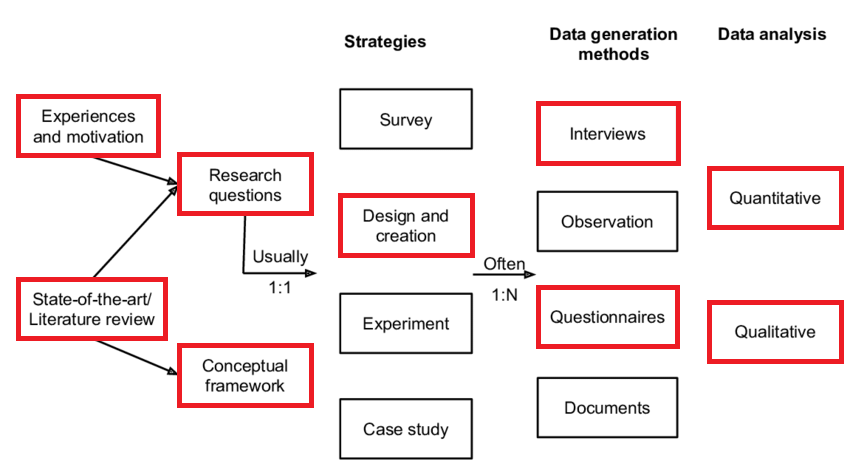
\includegraphics[width=\ImageWidth]{figures/oates_highlighted.png}
        \caption{Oates' Model of the Research Process}
        \label{fig:oates}
    \end{figure}
    \FloatBarrier
    
    The four first parts of the research process are stated to be more or less the same for all types of research. These are the four ''boxes'' to the left of \cref{fig:oates}: Experiences and motivation, Research questions, State-of-the-art/Literature review and Conceptual framework. The personal experience and motivation combined with a literature review create the research questions. The literature review also leads to the conceptual framework that \emph{''makes explicit how you structure your thinking about your research topic and the process undertaken''}. The remaining three categories have elements that can differ depending on the type of research. As indicated in the figure, one research question typically leads to one strategy, whereas a strategy can lead to several methods of data generation.
    
    \SPACE
    
    \subsection*{Research Method of this Master's Thesis}
    The research method was identified in the Specialisation Project\cite{specialisation}. This master's thesis conforms with Oates' model, with the four first parts present. This means that the project starts with existing experiences and motivation from the author. Combined with the literature review of the topic, research questions can be made. Additionally the conceptual framework of the terminology and relations take form and will be present throughout the thesis. The \textbf{Design and Create} strategy will be used to answer all of the presented research questions. This is done by developing the application, allowing it to be tested and compared to other applications.
    %Three data generation methods arise from the strategy: \textbf{Interviews}, \textbf{Observation} and \textbf{Questionnaires}. Students of the relevant course and domain experts will be invited to test the application. During these tests the users will be observed, then answer questionnaires and/or interviews.
    Two data generation methods arise from the strategy: \textbf{Interviews} and \textbf{Questionnaires}. People with VR equipment will be invited to download and test the \ApplicationName, whereas people without VR equipment will be supplied a video demonstrating the application. This video focused on showing the application as-is without explaining anything around it. This was to potentially uncover if anything in the application was unclear.
    Finally, the data analysis approach will be both \textbf{Qualitative} and \textbf{Quantitative}. The Questionnaires will be the main data source for the quantitative data analysis, whereas the interviews will supply data for the qualitative data analysis.
    
    \subsubsection{Questionnaire}
        The questions for the questionnaire were based on several other questionnaires with similar goals. Questions about individual differences, learning and enjoyment were taken from a study from Penn State in 2019 comparing the effect of virtual field trips to a control group \cite{transforming_earth_science}. Questions about control and active learning, and perceived learning effectiveness were taken from a study from 2010 investigating how desktop virtual reality enhances learning \cite{desktop_virtual_reality}. Questions about opinions on virtual field trips were taken from another Penn State paper from 2019 investigating virtual field trips in a geoscience course with elevated 360 degree images. The idea behind combining these questions is thoroughly investigate the learning and opinion aspect of the virtual field trip. The questions were used with a five point Likert scale \cite{likert} to create a quantitative and standardised data set.
        
        In addition to questions about learning, the System Usability Scale (SUS) \cite{sus} was used. This a relatively simple, but effective way of testing the usability of a system, using ten questions answered with a Likert scale. Questions from the User Experience Questionnaire (UEQ) \cite{ueq_questionnaire} were also included. These questions were meant to evaluate the application itself, not necessarily it's usefulness as a learning tool. The questionnaire can be viewed in \todo{import and reference questionnaire}.
        
    
    \subsubsection{Interview}
        The questions for the semi-structured interview were not taken from any literature, but created to find qualitative answers to the research questions. The questions were about evaluating the app itself and about virtual field trips and their possible usage in education. The questions for the interview can be viewed in \todo{import and reference interview}.

\section{Data Handling}
    % GDPR and group application from NSD
    % Questionnaire
    % Semi-structured interview
    When performing user tests, the data handling needs to be in accordance with the General Data Protection Regulation (GDPR)\cite{gdpr_eu}. In order to make sense of the regulations an article from \texttt{medium.com} detailing best practices of data handling was used. Following these practices, as little sensitive information as possible was collected. For the general questionnaires this meant none, focusing the questions on the application. The questions about the testers were also generalised, e.g. by placing them in age groups instead of asking for age. The questionnaire also avoided text answers, as this can be regarded as sensitive information.
    %For the semi-structured interviews, some personal information had to be kept. The practice of as-little-as-possible was still followed, and the interviews were recorded on non-internet connected devices, transcribed and anonymised.
    A group application was sent to the Norwegian Centre for Research Data to allow the collection of this data. 
    
    \todo{Update data handling after data has actually been handled}
    
    \begin{comment}
    \subsection*{Questionnaire}
        %The questionnaire was constructed to check which of the two applications the user tested and whether or not they had also tested the other.
        The questionnaire was constructed to check whether the tester had used the
        The users were also asked about their knowledge gain and how well they learned the area after using the application. Some questions from a short user experience questionnaire, provided by \texttt{ueq-online.org}\cite{ueq_questionnaire}, was used to assess the user experience of the applications. A question to investigate VR sickness was also added. The questionnaires were created using Google Forms\cite{google_forms}.
        %Online questionnaires have the issue of potentially logging the IP address of the user. This was circumvented by using one laptop for all the users, ensuring that IP addresses could not be linked to the answers. The questionnaire was also printed out to allow multiple users to answer at the same time. These questionnaires were then later added to the same database as the online questionnaire.
        
        \todo{Add questionnaire to appendix and cref}
        \todo{Avoided writing parts because of data handling}
    
    \subsection*{Semi-structured Interview}
    \end{comment}
        
\section{Changes due to Unforeseen Events}
    In the spring of 2020, the COVID 19 virus led to social distancing. This caused some changes to be made to the both the project and the application:
    
    \begin{itemize}
        \item \textbf{Testing} had to be done remotely instead of at the VR lab. The app had to be tested by however had VR equipment at home. Additionally a video demonstrating the application could be sent out to get feedback from those without VR equipment, especially students that attended the field trip in the autumn of 2019.
        
        \item \textbf{Focus} of the project had to be shifted from comparing two applications to evaluating one. This was because of the small possibility of people having two kinds of headsets available at home, the challenge of properly showing the differences via video, as well as reducing the extra work load introduced by the changes.
        
        %\todo{Other reasons? Possibility to capture footage from Oculus Go and make video?}
        
        \item \textbf{Teleporting} was added as an alternative way of movement in the \ApplicationName. This was to make it easier for home testing, both in development and evaluation, as very few people have a Virtuix Omni home.
        
        \item \textbf{Research questions} had to be changed late in the project. This mainly lead to removing a research question about how well the Virtuix Omni omnidirectional treadmill worked, as access to the lab was restricted. A new research question, R-5, was also added because of the changes to testing. By sending out a video and questionnaire, a broader audience was the data source, allowing to look at different opinions between geography students and the rest.
    \end{itemize}
    
    The changes also lead to delays in the progress plan, which will be discussed further in \todo{reference discussion: plan}.
    
\chapter{Background}
\label{chap:background}

\todo{Should information about the Vekveselva be included, or is it simply no interesting / important?}

\section{Theory and Technology}
    % About technology, both software and hardware that is currently on the market
    A literature review of the theory and technology of the field was conducted in the Specialisation project of which this master's thesis build. The following section is therefore directly extracted from said project\cite{specialisation}, with the exception of \cref{sec:threei}, \cref{sec:league} and \cref{sec:summary}\todo{Fill in cref} that have been added.
    
    \subsection{Different Types of Realities}
        % Continuum between real and virtual environment
        % Subgenres of extended reality XR
        When discussing different types of environments, it is natural to bring up the \emph{Reality - Virtuality continuum} \cite{reality_virtuality_continuum} as seen in \cref{fig:reality_virtuality_continuum}. This continuum was proposed in a paper by \emph{Paul Milgram} et al, discussing the different types of realities and environments.
        
        \begin{figure}[!ht]
            \centering
            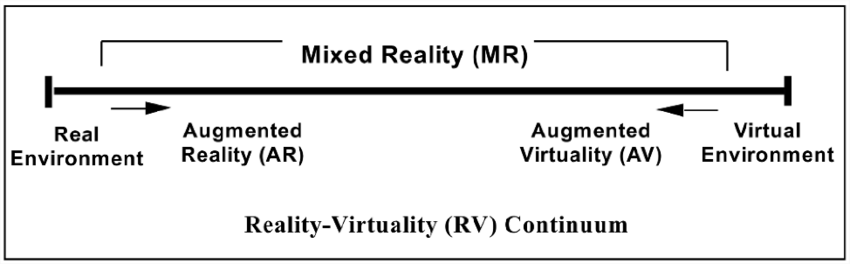
\includegraphics[width=\linewidth]{figures/reality_virtuality_continuum.png}
            \caption{The Reality - Virtuality Continuum}
            \label{fig:reality_virtuality_continuum}
        \end{figure}
        
        The continuum describes a continuous transition from the Real Environment, through the Mixed Reality into the Virtual Environment. Within the Mixed Reality there are two opposite realities: Augmented Reality (AR) and Augmented Virtuality (AV). Both include objects from the Real- and Virtual Environment, but differ in that AR is mainly the Real Environment with elements from the Virtual Environment, whereas AV is mainly the Virtual Environment with elements from the Real Environment. Because the transition is continuous it can become difficult to separate classify a reality as either AR or AV if it falls in between.
        
        \emph{Extended Reality} (XR) has been made as an umbrella term that incorporates both Mixed Reality and Virtual Reality \cite{xr}. This has been done to make a separation between the Real Environment and the rest that have some form of technology involved. The hierarchical relations of the different realities and environments have been illustrated in \cref{fig:xr}.
        
        \FloatBarrier
        \begin{figure}[!ht]
            \centering
            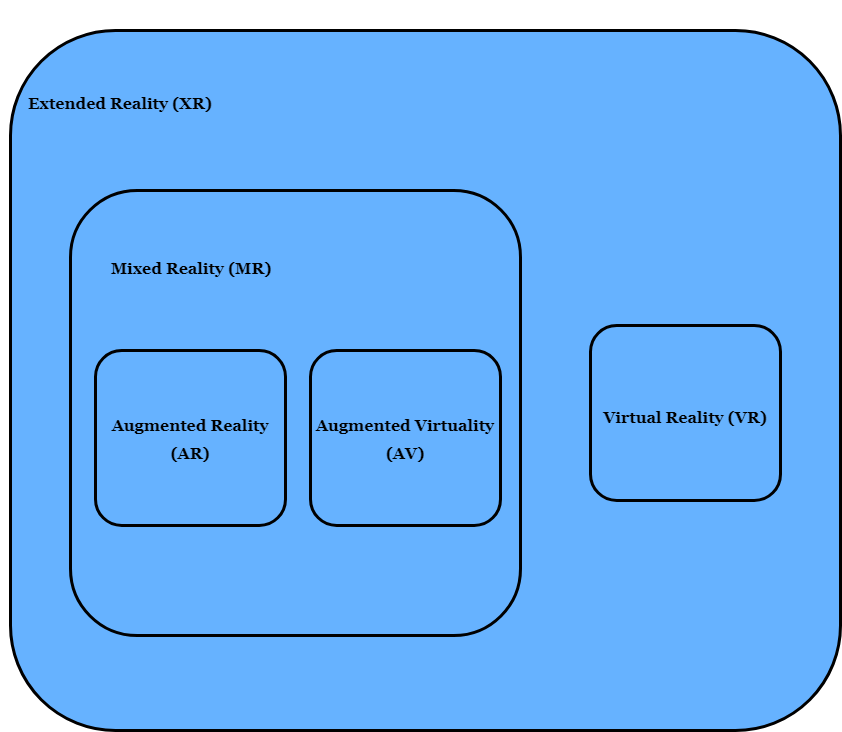
\includegraphics[width=0.7\linewidth]{figures/XR.png}
            \caption{Categories of Extended Reality}
            \label{fig:xr}
        \end{figure}
        \FloatBarrier
        
        As the Virtual Field Trip is planned to rely on a Head Mounted Display and the Omnidirectional Treadmill without using real elements directly, it will fall under the category of VR.
    
    \subsection{Virtual Reality}
        Even though Virtual Reality (VR) has become part of the mainstream media market, a brief introduction and evaluation is presented here.
        
        According to the Oxford Dictionary \cite{oxford}, VR is:
        
        \begin{quote}
            \textit{''The computer-generated simulation of a three-dimensional image or environment that can be interacted with in a seemingly real or physical way by a person using special electronic equipment, such as a helmet with a screen inside or gloves fitted with sensors.''}
        \end{quote}
        
        Another dictionary, Merriam Webster \cite{merrian_webster}, defines VR as:
        
        \begin{quote}
            \textit{''An artificial environment which is experienced through sensory stimuli (such as sights and sounds) provided by a computer and in which one's actions partially determine what happens in the environment''}
        \end{quote}
        
        In the book \emph{The VR Book} by Jason Jerald \cite{the_vr_book}, VR is defined as:
        
        \begin{quote}
            \textit{''[...] a computer-generated digital environment that can be experienced and interacted with as if that environment were real.''}
        \end{quote}
        
        The definitions start to paint a picture of VR. A common denominator between these is a \textbf{computer-generated environment}. Furthermore they all agree on this environment being \textbf{interactive}.
        
            \subsubsection{The Three I's of VR}
                \label{sec:threei}
            
                \FloatBarrier
                \begin{figure}
                    \centering
                    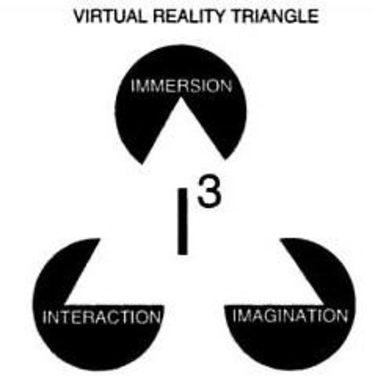
\includegraphics[width=0.5\linewidth]{figures/three_i.png}
                    \caption{The Three I's of Virtual Reality}
                    \label{fig:three_i}
                \end{figure}
                \FloatBarrier
                
                The term VR is also explored in the book \emph{Virtual Reality Technology}\cite{threei}. It is stated that VR has the three features: Immersion, Interaction and Imagination. As seen in \cref{fig:three_i}, the features are represented as equally important to the nature of VR. The book defines VR as:
                
                \begin{quote}
                    \textit{''Virtual reality is a high-end user-computer interface that involves real-time simulation and interactions through multiple sensorial channels. These sensorial modalities are visual, auditory, tactile, smell and taste.''}
                \end{quote}
                
                From this definition, the Immersion and Interaction feature of VR are clearly rooted. An important point made by the book is that VR should not be defined based on the devices that are used, but rather its purpose and function. The last feature, Imagination, is less obvious at first glance. Although not directly present in the quoted definition, VR is not only an interface, but has applications for real life problems. Because of this the imagination of the user is important for the performance of the simulation, and therefore the extent of which the application can solve a real problem. The imagination is also necessary to perceive non-existing things. This an important point as VR, although immersive, can not perfectly simulate the reality. The imagination bridges this gap by letting the user invest themselves in the simulated world, not unlike the suspension of disbelief when reading a book or watching a theatre play. This is demonstrated by the perceived, non-existing triangle in \cref{fig:three_i}.
                
                \todo{Cannot vs can not?}
                
            \subsubsection{VR Sickness}
                % Theories on why
                An unfortunate side effect that can arise from VR is VR sickness. VR sickness manifests itself in the same way as motion sickness, and can case nausea, vomiting and trouble maintaining balance \cite{motion_sickness}. According to researchers from the University of Newcastle Australia \cite{vr_sickness}, motion- and VR sickness might be the same thing, although other studies disagree. In the University of Newcastle study the researchers exposed volunteers to uncomfortable physical and visual tests and found large similarities in how the volunteers reacted. As the nature of VR- and motion sickness is still debated, there are a few theories to the cause of the problem \cite{vr_sickness_theories}:
                
                \begin{itemize}
                    \item \textbf{Sensory Conflict Theory} \\
                    This theory is the most widely accepted and states that the sickness is caused by a mismatch between visual and physical input. This happens when the eyes perceive motion, especially acceleration, and the body senses no force acting upon it.
                
                    \item \textbf{Eye Movement Theory} \\
                    The theory suggests that the eyes move unnaturally compared to real life when viewing in \emph{Head Mounted Displays}. This happens because the images change differently to what the eyes expect and therefore strains the eyes, causing discomfort.
                    
                    \item \textbf{Postural Instability Theory} \\
                    This theory builds on the theory that sickness occurs when animals are unable to keep their posture \cite{postural_instability}. On the assumption that this is correct, VR sickness is explained by small subconscious actions done to anticipate movement shown visually that is not present physically. These actions throw the user of balance, disrupting the posture and causing discomfort.
                    
                    \item \textbf{Evolutionary Theory} \\
                    This is not as much a separate theory as more of a possible explanation of \emph{why} the sickness is present. It states that the symptoms are evolutionary reactions made to survive poisoning that can cause mismatch between visual and physical impressions, which is a common denominator in the different theories.
                \end{itemize}
                
                Regardless of the true reason for VR sickness, the theories provide similar ways to avoid it. The main points are to keep the players as stable as possible, avoiding acceleration and providing stable frames of references to help orient them.
            
        \subsection{VR, Learning and Engagement}
            As the presence of XR equipment increases, so too does the available research and experience with the technology. Several research papers have emerged that regard XR as improving learning outcome compared to traditional methods, like reading books and articles.
            
            A. Vishwanath et Al \cite{vr_low_income} studied the introduction of learning with VR by using Head Mounted Displays in a learning centre in a low income area in India. They worked with 16 students for several weeks, creating VR applications that covered several fields of study. They observed that the use of VR lead to the students displaying more curiosity in the field and being more inquisitive.
            
            D. M. Markowitz \cite{virtual_field_trips_learning} performed studies, field studies and experiments on over 270 students. They also noted that students were more curious after being exposed to VR learning applications as well as more knowledgeable. They also found a correlation between how much the students explored the space of the VR applications and how curious and inquisitive they became of the subject. This can be an indication that a more engaging experience offers better learning and sparks curiosity.
        
        \subsection{Head Mounted Displays}
            As the project will only include VR from the Reality - Virtuality Continuum, it will, as VR for the largest part does, be based on Head Mounted Displays. Generally speaking these are headsets that contain one or two screens and lenses capable of projecting individual images to each eye. The new application will use the HTC Vive Pro, whereas the Penn State application runs on the Oculus Go.
                
                \subsubsection{HTC Vive Pro}
                    This headset setup consists of two base stations, two controllers and the headset itself. The base stations are installed in a room to accurately track the players head and hand movements. It is not a stand-alone Head Mounted Display, and must therefore be connected and run on a computer. The headset has a resolution of 1440 x 1600 per eye on dual AMOLED screens, adding up to a total of 2880 x 1600. It Has a refresh rate of 90Hz and includes an integrated microphone and headphones. It won the award ''VR Headset of the year'' in 2018 and can be regarded as high-end hardware. \cite{vive_pro}
                    
                    \FloatBarrier
                    \begin{figure}[ht]
                        \centering
                        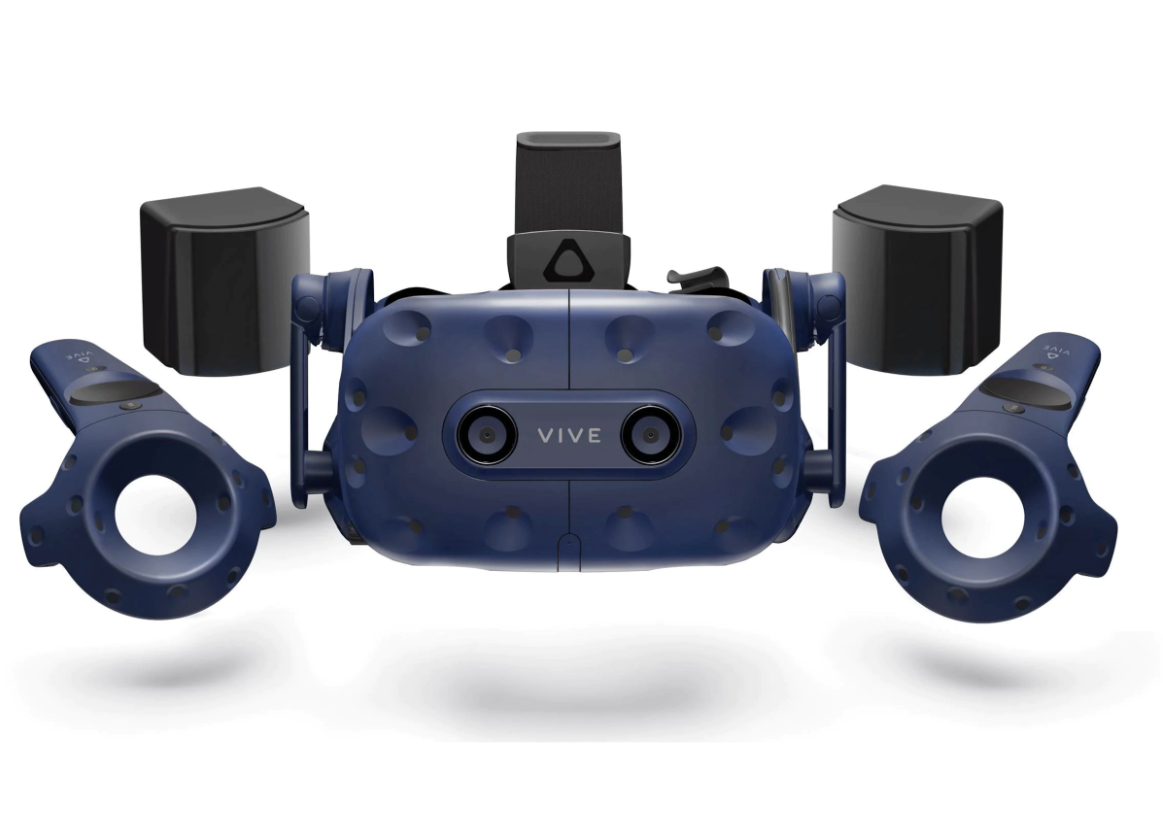
\includegraphics[width=0.9\linewidth]{figures/vive_pro.PNG}
                        \caption{The HTC Vive Pro Head Mounted Display with controllers and base stations}
                        \label{fig:vive_pro}
                    \end{figure}
                    \FloatBarrier
                    
                \subsubsection{Oculus Go}
                    In contrast to the HTC Vive Pro, the Oculus Go is a stand-alone Head Mounted Display, meaning that it has internal processors and does not need to be connected to a computer. It consist of one headset and one controller. It also has integrated speakers to offer an audible experience\cite{oculus_go}. This means that is a lot more portable and easier to set up, but at the cost of lower processing power and less accurate controller tracking. The Oculus has one 538 ppi\footnote{pixels per inch} screen with a resolution of 2560 x 1440\cite{oculus_specs}. It was launched in 2018, so it is from the same era as the HTC Vive Pro, but with a different purpose and price range.
                    
                    \FloatBarrier
                    \begin{figure}[ht]
                        \centering
                        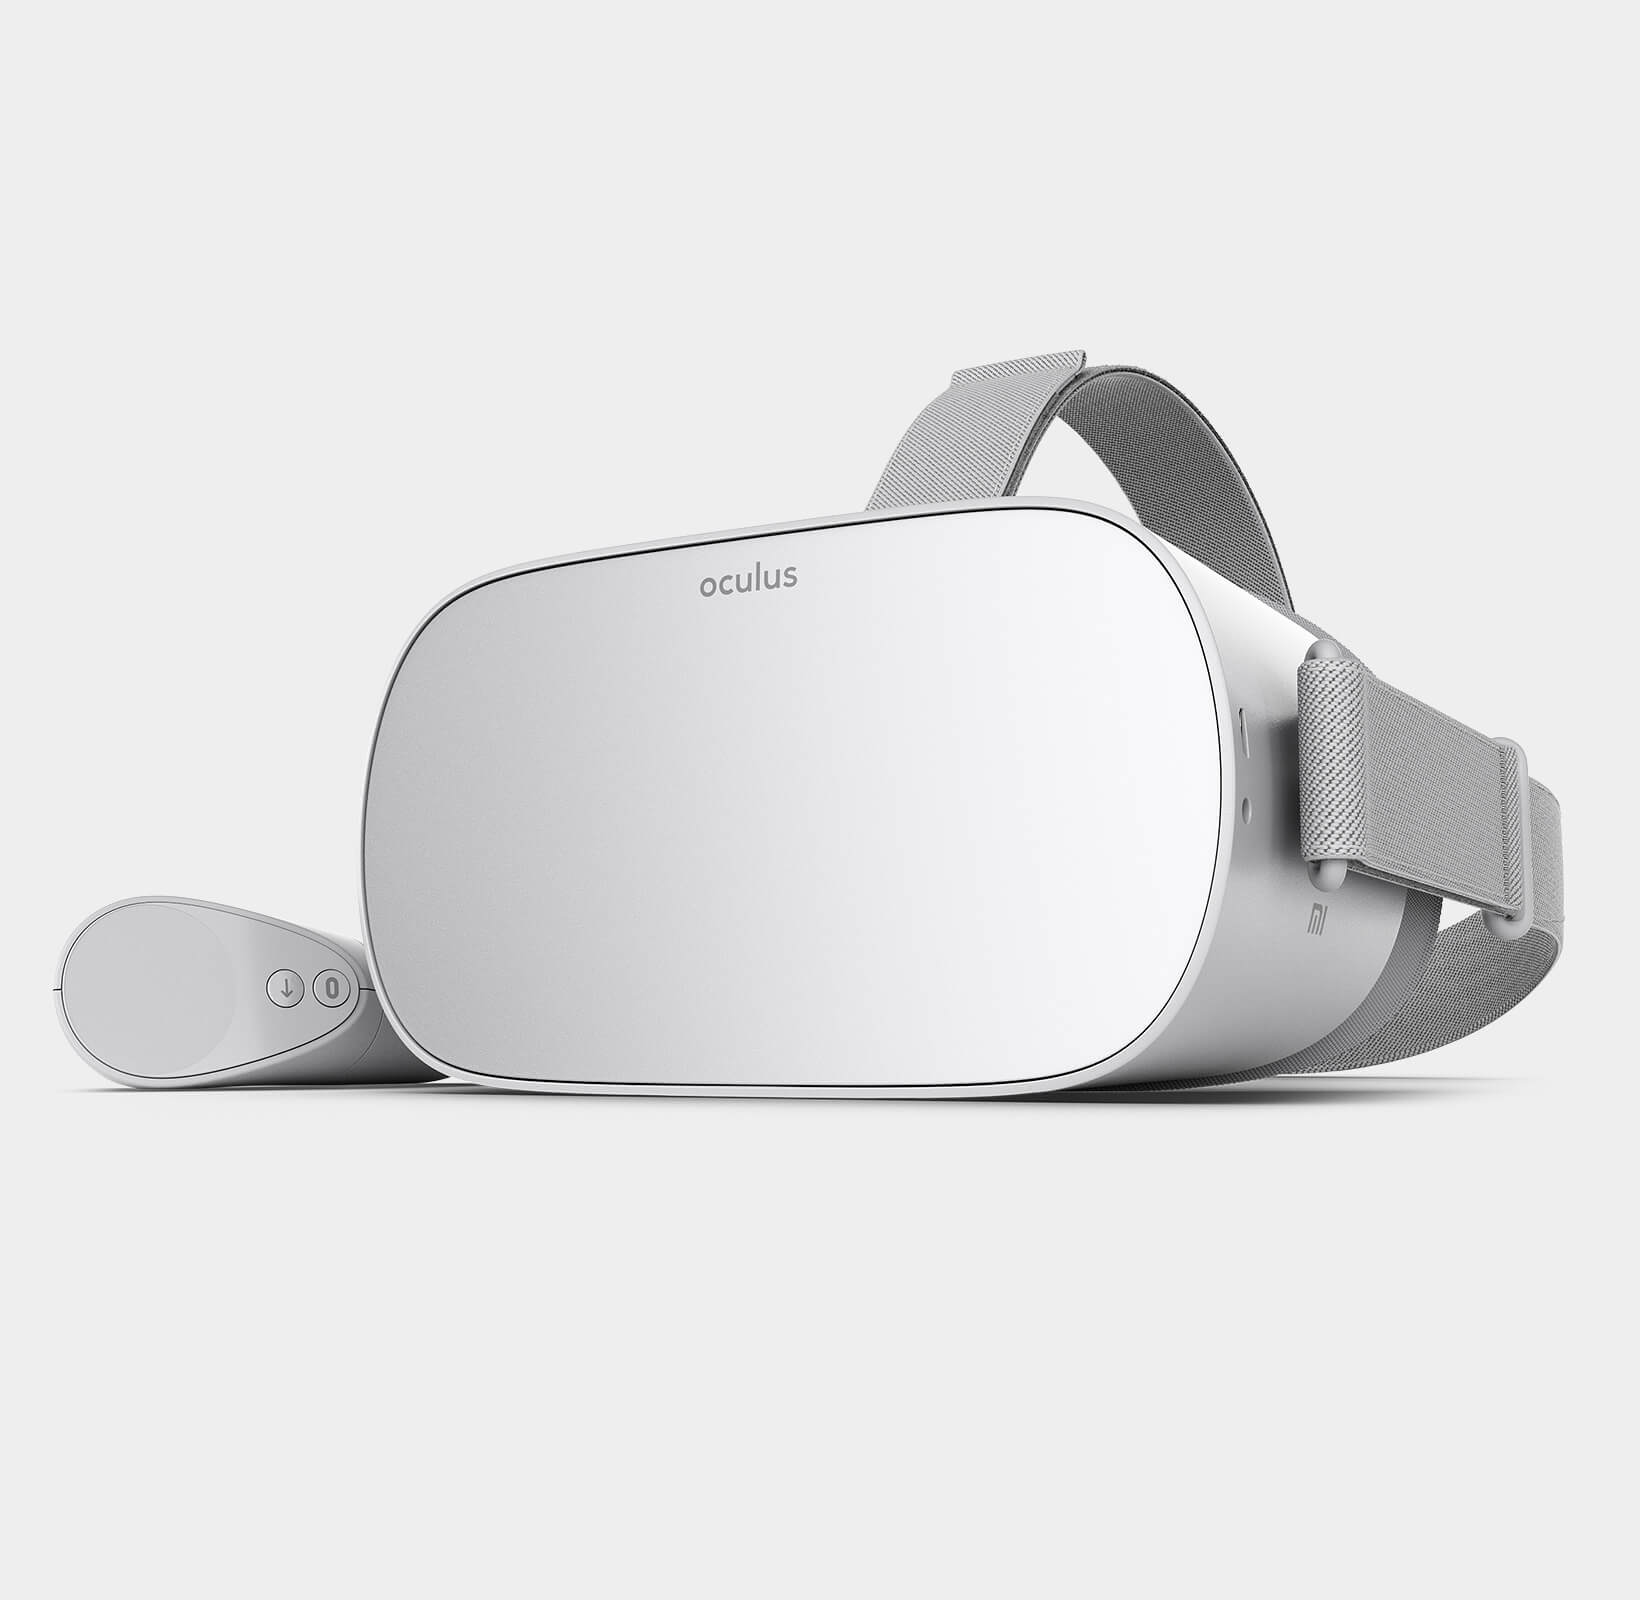
\includegraphics[width=0.9\linewidth]{figures/oculus_go.jpg}
                        \caption{The Oculus Go Head Mounted Display with its controller}
                        \label{fig:oculus_go}
                    \end{figure}
                    \FloatBarrier
                
                \todo{About Oculus Quest in case it will be used. Is that just unnecessary introduction of variables?}
            
            \subsection{Omnidirectional Treadmill}
            \label{sec:omni}
            
            \FloatBarrier
            \begin{figure}[!ht]
                \centering
                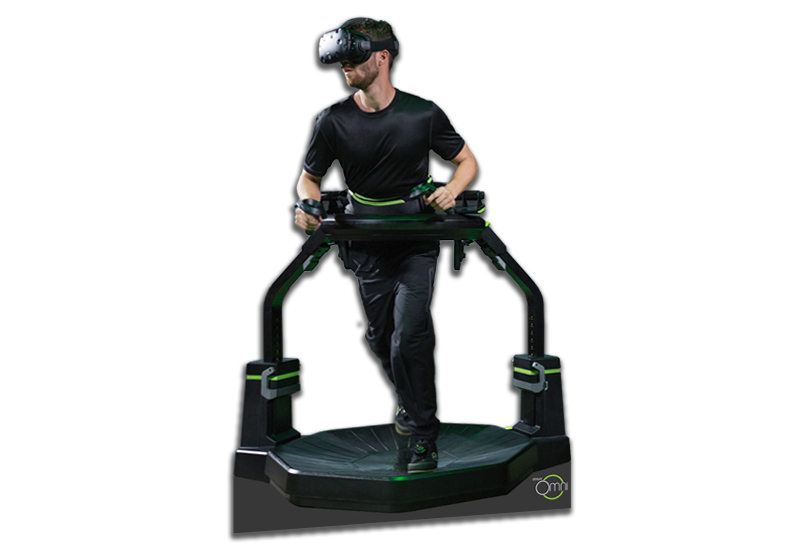
\includegraphics[width=0.9\linewidth]{figures/omni.png}
                \caption{Omni - the Omnidirectional Treadmill by Virtuix}
                \label{fig:omni}
            \end{figure}
            \FloatBarrier
            
            The Omni is an Omnidirectional Treadmill developed by Virtuix \cite{omni} and will be used as hardware for movement for the new application in the project. It is compatible with the HTC Vive Pro head mounted display. As illustrated in \cref{fig:omni} it consists of a concave surface, low friction shoe covers and a harness to keep the player in place. The Omni tracks the orientation of the player from the harness, as well as the feet movement by wireless sensors connected to the shoe covers. The movement of the feet is then transformed to in-game motion. The Omni can be used by an SDK\footnote{Software Development Kit} \cite{omni_sdk}, and Virtuix supplies SDKs for both the Unity and Unreal game engine. From Omni's web pages it can be seen that the applications featured are all of the entertaining type. This is indicative of it being mainly used for games and not for education.
    
    \subsection{Virtual Field Trips}
        Virtual Field Trips (VFTs) are becoming more common in STEM\footnote{Science, Technology, Engineering and Math} education, where the areas of study that most implement the Virtual Field Trips are geography, geoscience and architecture. Virtual Field Trips are, as the name implies, simulations of field trips meant to either support or replace the actual field trip. Even though they become more prominent, there are still numerous constraints to creating and using these applications, where many of the constraints revolve around the lack of tools that allow domain experts to create the Virtual Field Trips themselves\cite{vft_geoscience}. Despite these challenges, some evidence point towards the Virtual Field Trips having positive impacts on the courses. Research and experiments done by Kathy Jackson et al \cite{ivft_effectiveness} at Penn State University states that other research done on the effectiveness have shown inconsistent result, whereas they themselves found very positive impact on learning, enjoyment and grades. The inconsistent results can indicate that the topic needs more research.
    
    \subsection{VR Virtual Field Trips}
        Virtual Field Trips are not necessarily in VR, but VR is the focus of this master's project. The current trend when it comes to the use of VR Virtual Field Trips is to use \emph{low-level} VR applications, meaning VR applications that run on low-cost hardware and that can be created with relatively low cost, effort and VR expertise \cite{vr_low_cost}. An opportunity that is present in these low cost VR applications is to have multiple users experiencing the field trip at once. This is something that can be taken into account when implementing non-low cost applications, as they will likely be used with an audience of other students.
    
    \subsection{Framework for Evaluating Virtual Field Trips}
        \label{sec:framework}
        In their research article, A. Klippel et al \cite{research_framework} propose a framework for assessing immersive learning experiences, specifically \emph{immersive Virtual Field Trips} (iVFTs). In essence this framework is a two-dimensional plane where one rates the VR technology on one axis and the content of the Virtual Field Trip on the other axis. An overview of the research framework is presented in \cref{fig:framework}
        
        \FloatBarrier
        \begin{figure}[!ht]
            \centering
            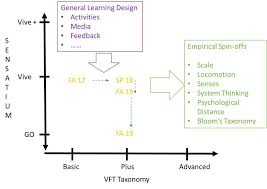
\includegraphics[width=0.7\linewidth]{figures/framework.jpg}
            \caption{Overview of the Research Framework for Immersive Virtual Field Trips}
            \label{fig:framework}
        \end{figure}
        \FloatBarrier
        
        On the left, vertical axis of the research framework overview (\cref{fig:framework}), the VR technology is evaluated. \emph{SENSATIUM} is a term coined by A. Klippel et al, which is an acronym for the \textbf{SEN}sing - \textbf{S}c\textbf{A}lability \textbf{T}rade - off cont\textbf{I}nu\textbf{UM}. As seen in \cref{fig:sensatium}, \emph{SENSATIUM} is a continuous scale where scalability goes from high to low, and sensing goes from low to high. Both are dependant on how advanced the equipment is. This shows that higher levels of sensing typically trades off against the ability to scale the application.
        
        \FloatBarrier
        \begin{figure}[!ht]
            \centering
            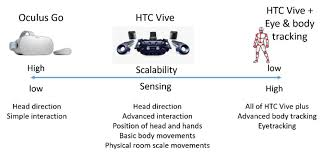
\includegraphics[width=0.7\linewidth]{figures/framework_technology.jpg}
            \caption{SENSATIUM, the \textbf{SEN}sing - \textbf{S}c\textbf{A}lability \textbf{T}rade - off cont\textbf{I}nu\textbf{UM}}
            \label{fig:sensatium}
        \end{figure}
        \FloatBarrier
        
        On the horizontal axis of the research framework overview (\cref{fig:framework}) the content of the immersive Virtual Field Trip is evaluated. The continuous scale goes from \emph{Basic}, through \emph{Plus} to \emph{Advanced}. This rating of immersive Virtual Field Trips, called the \emph{taxonomy} of immersive Virtual Field Trips, was also established by A. Klippel et al. The \emph{taxonomy} is explained in \cref{fig:taxonomy}
        
        \FloatBarrier
        \begin{figure}[!ht]
            \centering
            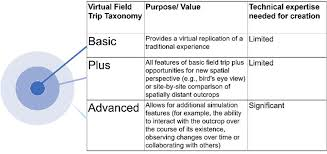
\includegraphics[width=0.7\linewidth]{figures/framework_content.jpg}
            \caption{Taxonomy of Immersive Virtual Field Trips}
            \label{fig:taxonomy}
        \end{figure}
        \FloatBarrier
        
        The different levels of Virtual Field Trips are explained in the figure, but can be summed up as Basic being replication of a real field trip, Plus adding new spatial perspective and Advanced adding simulations and / or models, allowing access to realities that does not exist in the real field trip.
        
    \subsection{The LEAGUE Framework for Evaluation}
        \label{sec:league}
        The LEAGUE framework\cite{league} was developed to simplify the evaluation of game-based learning. The framework was created by reading literature on the topic and extracting common features. The features were then placed in a three level hierarchy. The gist of the framework is that game-based learning can be divided into six dimensions (that make up the name LEAGUE): \textbf{L}earning, \textbf{E}nvironment, \textbf{A}ffective Relations, \textbf{G}ame Factors, \textbf{U}sability and Us\textbf{E}r. These dimensions are then further decomposed into factors and sub-factors. Finally, the sub-factors can be evaluated through metrics. The metrics is the lowest level in the model and the parts that can actually be compared. The five metric types are: scores, time, number of occurrences, rating or opinions. The idea of the framework is to use this hierarchical model when planning, designing and evaluating games to ensure a universal language. An overview of the hierarchy is presented in \cref{fig:league}:
        
        \FloatBarrier
        \begin{figure}[htbp]
            \centering
            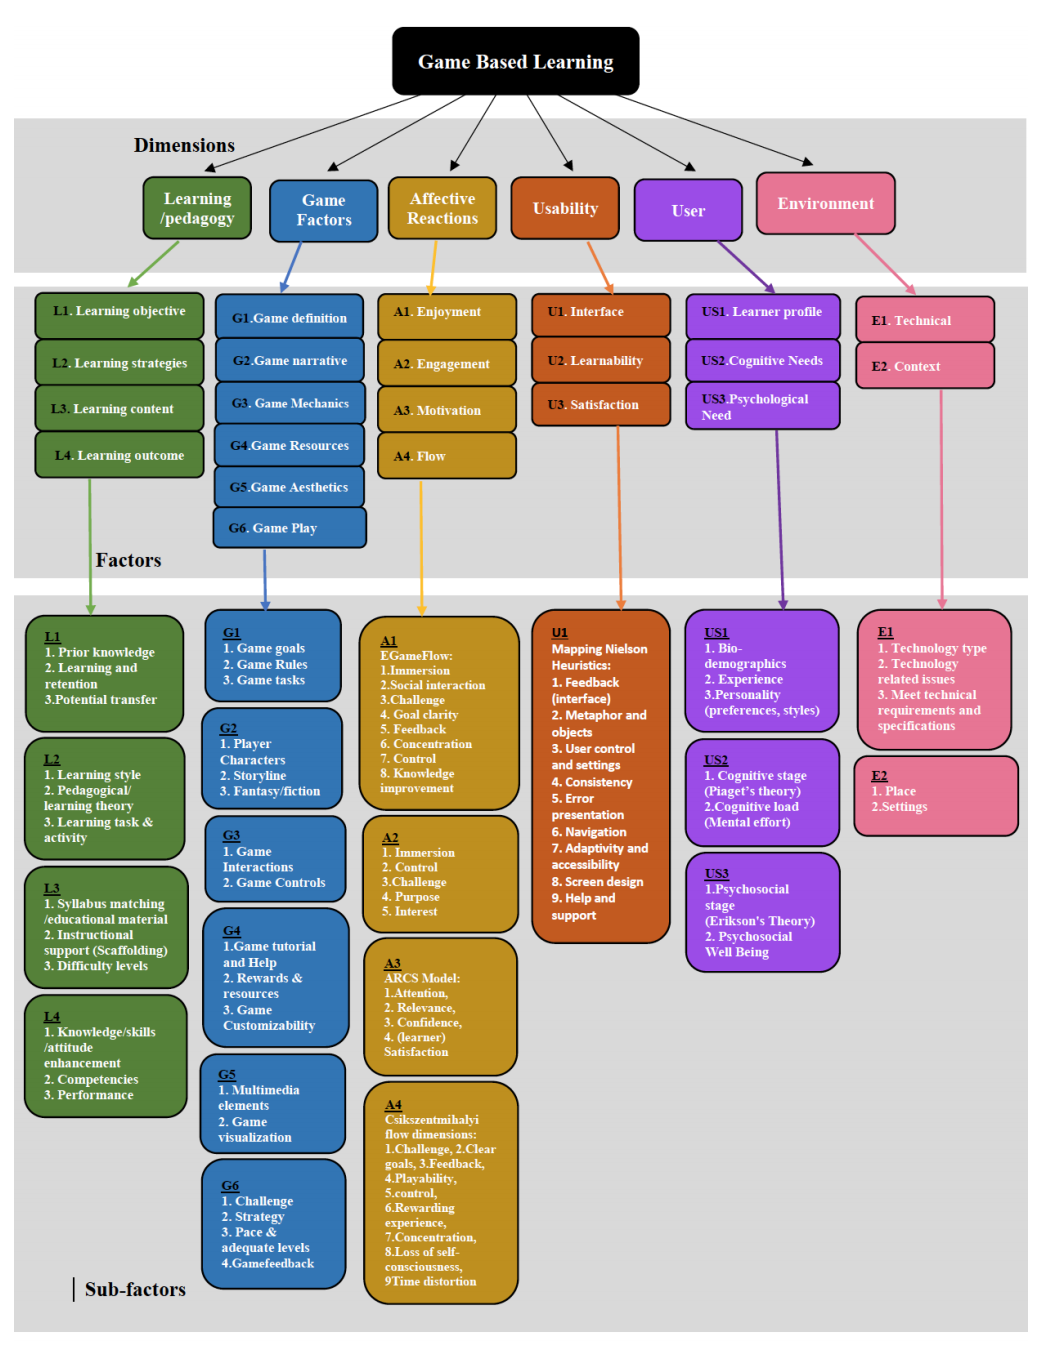
\includegraphics[width=\ImageWidth]{figures/league.PNG}
            \caption{LEAGUE Hierarchical Structure and Components}
            \label{fig:league}
        \end{figure}
        \FloatBarrier
        
    \subsection{LiDAR}
        A LiDAR scanner is a Light Detection And Ranging equipment that can record the surface area of objects \cite{lidar}. The LiDAR consists of a laser emitter to send laser pulses, a scanner to precisely record the reflected laser pulses, and a GPS receiver to accurately track the position of the LiDAR equipment during scanning. By very precisely recording the time between laser pulses that are sent out and reflected back, the speed of the pulses (light speed) can be used to calculate the distance between the LiDAR and the object reflecting the laser. By repeating this process of sending and detecting laser pulses in different directions, a point cloud will be generated that represent the surface area of the object. Because of the GPS receiver the LiDAR can be moved during scanning, which allows for aerial scanning from helicopters and planes.
        
        LiDAR equipment can be divided into two categories depending on the laser type they use to scan the surfaces. \emph{Topographic} LiDAR systems uses near-infrared lasers. This type of laser will, as explained above, be reflected by surfaces and give a point cloud reminiscent of what one would see from the point of view of the LiDAR. \emph{Bathymetric} LiDAR uses a green light laser. This laser is better at penetrating water, opening the possibilities for mapping sea- and riverbeds where the topographic LiDAR would only return the surface of the water.
        
        As LiDAR equipment bases its sensoring on laser pulses it can also exploit one of the properties of light: not everything is reflected\cite{lidar_canopy}. Illustrated in \cref{fig:transmission} is the effect when some of the light from the LiDAR is reflected back while the rest continues, penetrating through the object or missing it entirely. This is especially common in vegetation, as leaves are thin and do not cover the entire area. This allows one pulse to give multiple readings, which can be used to gather information about the vegetation itself or filter it out to get an isolated view of the ground.
        
        \FloatBarrier
        \begin{figure}[ht]
            \centering
            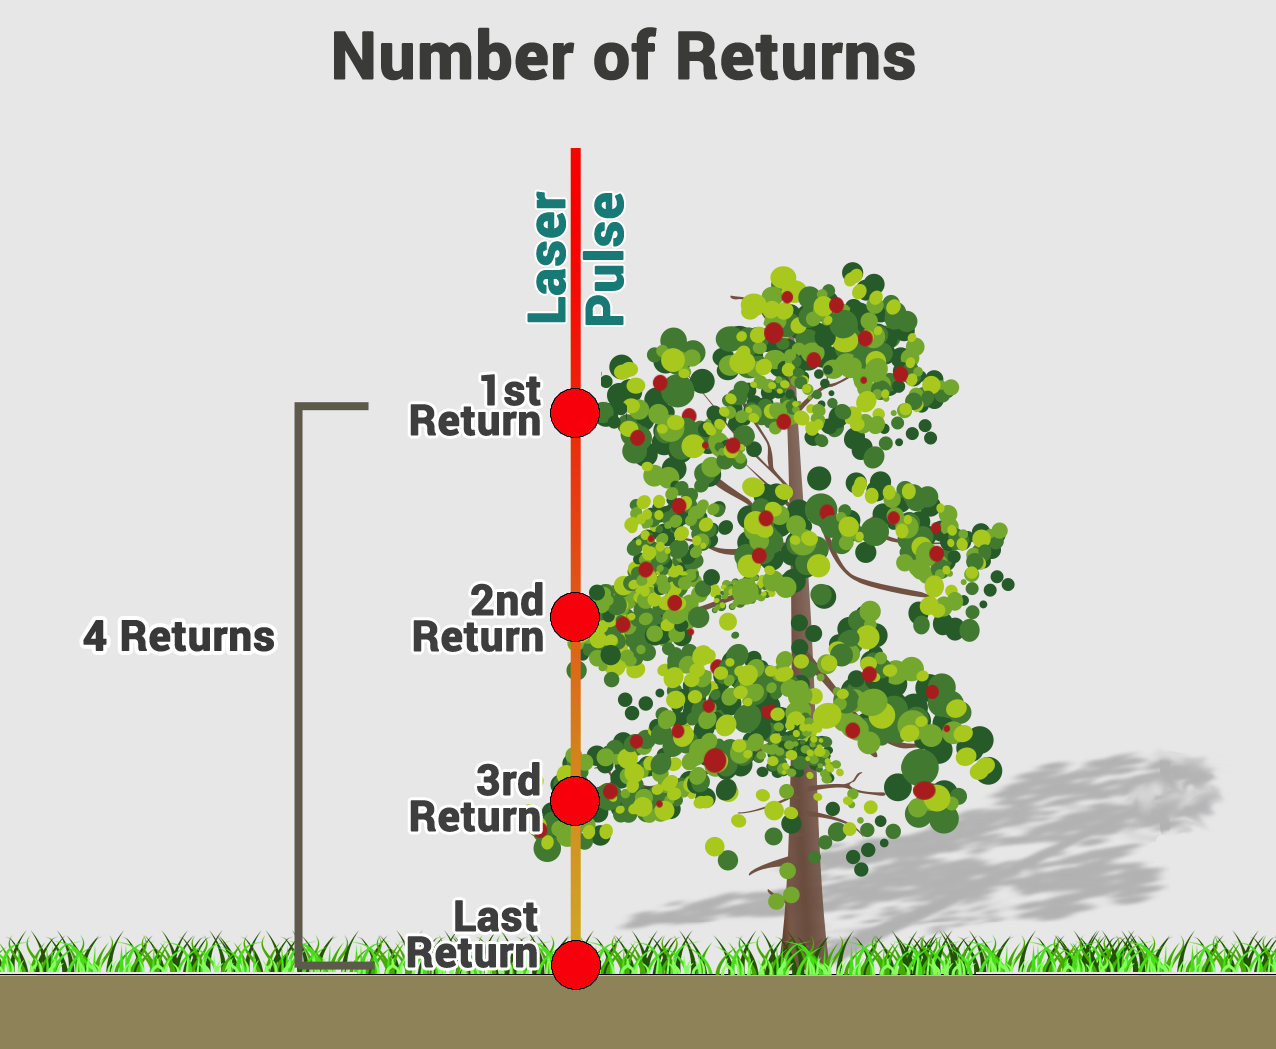
\includegraphics[width=0.5\linewidth]{figures/lidar.png}
            \caption{Laser pulses partially reflecting on- and penetrating canopy}
            \label{fig:transmission}
        \end{figure}
        \FloatBarrier
        %It does this by sending out laser pulses and record the time when they are reflected back in order to determine the distance to a point on a surface. By repeating this process a point cloud can be constructed. LiDAR equipment also record the GPS location for each pulse, which makes it possible to move the scanner during recording and thus open up the possibilities of aerial scans using planes.
        
\section{Game Design}
\label{sec:game_design}
    As the new application is planned to contain interactive elements and meant to be engaging, some theories from Game Design are presented. These are theories and heuristics for creating good games in general, as well as more specific theory related to educational games, which one can argue also adhere to Virtual Field Trips.
        
    \subsection{Lazzaro's Four Fun Keys}
        In chapter 20 of the book \emph{Game Usability: Advice from the Experts for Advancing the Player Experience}\cite{lazzaro}, Lazzaro presents the theory that there are four types of fun to be found in video games. She goes on to describe that players have a tendency to transition between three of these, which implies that successful games have at least three of the four types of fun present to cater to the players desires throughout the gaming sessions. The four types of fun are:
        
        \begin{itemize}
            \item \textbf{Hard Fun}\\
            This is the type of fun most people think of when talking about video games: the fun of the challenge. It is explained that the Hard Fun follows a cycle where the player meets a challenge and builds up frustration, followed by a phase named \emph{Fiero!} when the player overcomes the challenge. Afterwards comes a phase of relaxation where the player can bask in the glory of their achievements before the cycle starts again. It is important that the challenge is correctly balanced to give the player the right amount of frustration before the \emph{Fiero!}. It is also important to allow the player to ''cool down'' before starting to build up more frustration.
            
            \FloatBarrier
            \begin{figure}[ht]
                \centering
                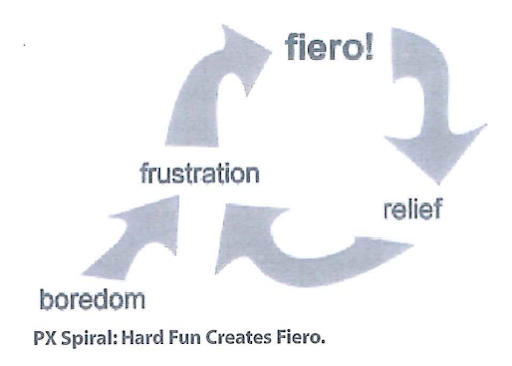
\includegraphics[width=0.5\linewidth]{figures/hard_fun.png}
                \caption{The Hard Fun Cycle}
                \label{fig:hard_fun}
            \end{figure}
            \FloatBarrier
            
            \item \textbf{Easy Fun}\\
            This type of fun is connected to the story and the wonders of the world within the game. It is the type of fun one have when exploring mystic worlds or the curiosity when trying to uncover the hidden story of a forgotten incident. Like the Hard Fun, Easy Fun is also a cyclic behaviour where curiosity leads to a surprise that causes wonder. This is followed by a cool-down phase of relief before the cycle continues. Also similar to Hard Fun, the surprise in Easy Fun must be balanced in order to keep the content familiar enough to be engaging, but also surprising enough.
            
            \FloatBarrier
            \begin{figure}[ht]
                \centering
                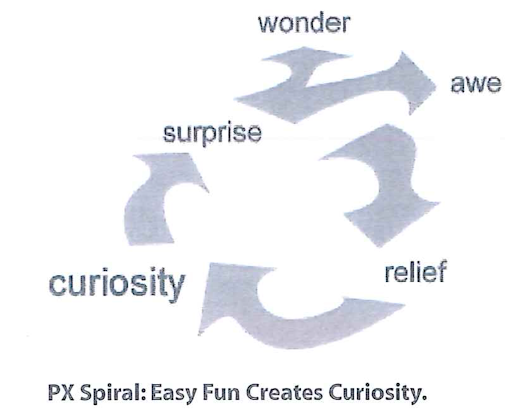
\includegraphics[width=0.5\linewidth]{figures/easy_fun.png}
                \caption{The Easy Fun cycle}
                \label{fig:easy_fun}
            \end{figure}
            \FloatBarrier
            
            \item \textbf{Serious Fun}\\
            This type of fun is defined as when the game ''create something of value outside of the game itself''. Examples of this can be to use games to relax after a hard day at work, to learn rhythms or, in our case, to learn something. Serious Fun can lead to more motivation as the game is not just played for fun, but can improve the player in some way.
            
            \item \textbf{People Fun}\\
            People Fun is the fun related to the social aspects of games. This type of fun is very obvious in multiplayer games with both cooperative and competitive interaction between the players. It does however not explicitly require other players, as it can also be achieved through the use of Non-Player Characters (NPCs).
        \end{itemize}
        
    \subsection{Heuristics For Designing Instructional Computer Games}
        A set of heuristics for designing instructional computer games are given by Malone in his article from 1980\cite{heuristics}. The heuristics describe essential characteristics divided into three categories:
        
        \begin{itemize}
            \item \textbf{Challenge}\\
            Similar to Lazzaro, Malone states that an instructional game must be challenging. He goes forth to describe heuristics for the goal that shall be completed, stating that it should be:
            
            \begin{itemize}
                \item Obvious
                
                \item Compelling
                
                \item Of the appropriate difficulty
                
                \item Offering performance feedback
            \end{itemize}
            
            By following this heuristic the player should end up with knowing what to do, as well as having a motivation for doing it. It should be within the players ability to do it, and they should have a clear indication of how well they perform, both when under- and over performing.
            
            In addition to the goal, the game should have an uncertain outcome. This is to ensure that it becomes exciting, as a game where one always win or always lose can quickly become boring. This uncertain outcome can be achieved by having:
            
            \begin{itemize}
                \item Variable difficulty setting
                
                \item Multiple level goals
                
                \item Hidden information
                
                \item Some randomness
            \end{itemize}
            
            The difficulty can be set manually by the player, or be set automatically by the performance of the player. The difficulty is important as it can greatly affect the self-esteem of the player, which again will influence motivation. Having multiple level goals is another way to balance the difficulty, by making obligatory tasks of the goal easy, but offering challenging optional goals. The hidden information is also a great way to make the outcome of the challenge uncertain by revealing information along the way. Randomness can both aid the hidden information, as well as increasing the difficulty.
            
            \item \textbf{Fantasy}\\
            Fantasy in games can be used to make them more compelling, but can also be used as a means of challenge by having tasks that require players to use their fantasy. An important note is that different fantasies are compelling to different people, and should therefore be chosen based on the target audience.
            
            Malone differs between two different kinds of fantasies: extrinsic and intrinsic. The extrinsic fantasy is dependent on the player skill, where the example in the article is the game Hangman where the visuals depend on the actions of the player. The extrinsic fantasy is also dependant on the skill, but the skill is also dependant on the fantasy. This means that the fantasy is used together with the skill. The example here is a game of darts where the trajectory, angles and force must be fantasised by the player, thus being used in conjunction with the skill.
            
            Emotion is also discussed under the Fantasy category. It is a very powerful element, but it is also very hard to use. By emotionally engaging the player with e.g. NPCs in the game, the goal can be perceived as more compelling, and the feedback will have a stronger impact on the player. Because of the difficulties of using emotion, there are no general way to approach this element.
            
            \item \textbf{Curiosity}\\
            Curiosity mainly stems from having the right amount of \emph{informal complexity}. The goal is to have the player comprehend the situation, but also having some uncertain or hidden information. Curiosity is divided into two categories: sensory and cognitive. The sensory curiosity instinctively captures the players attention, usually by playing visual or audible ques. This plays on the ''lizard brain'' of humans that automatically seeks out movement and flashing lights. The cognitive curiosity however relies on missing information. This has some similarities with Lazzaro's Easy Fun in that the missing information should be surprising to engage the player and motivate further progress.
        \end{itemize}

\section{Existing Solutions}
    % Products of Virtual Field Trips that are available to be used atm
    
    \todo{Include images of applications?}
    
    As discussed in \cref{sec:motivation}, virtual field trips using VR is already present and available as commercial products. A quick introduction to some of the most similar or relevant solutions are presented, as well as summary comparing the different applications on key factors. Applications are chosen based on the criteria below, where the first is mandatory and at least one of the other two must be present.
    
    \begin{itemize}
        \item \textbf{Application have to be in VR}
        
        \item Application is a Virtual Field Trip
        
        \item Applications uses an omnidirectional treadmill
    \end{itemize}
    
    \subsection{Penn State University Application}
        Penn State University has created an application for showing images taken from a field course. The application provides the player with an aerial map of the area where image locations are highlighted. Players can then select images from the map, from a menu available when in image mode and by using arrows within the image to move to adjacent images. The application only support monoscopic 360 images, limited by the intended hardware: Oculus Go and Oculus Quest. The application does allow for multiple users at the same time, where one of the users can guide the other users through the images while explaining the content.
        
        This is the Virtual Field Trip that will be used to compare and evaluate the new application. It has been made in collaboration with Penn State. Specifications for how to capture and mark the footage was supplied from Penn State and the images were sent back in monoscopic format, geotagged and with indications of which images transition to which. The development was incremental with a prototype being tested on domain experts and reworked based on their feedback.
    
    \subsection{Google Expedition}
        % Phone app
        % VR and AR
        % One leader can see where other participants are seeing
        % "Go anywhere with VR, see anything with AR"
        % Create own virtual tours with Tour Creator
        Google Expedition is a smart phone application available on both Google Play and the App Store. As can be read on Google's own pages about the product \cite{google_expeditions}, the application offers both VR and AR functions. When used as VR, one leader can guide others through 360 images and see where the participants are looking. When using the AR functionalities, objects can be displayed and viewed from all angles making the participants walk around a fixed physical location in the classroom.
        
        Google Expedition also has the ability for domain experts to create their own Virtual Field Trips with the Tour Creator. It can create tours from 360 images, 180 images or images from Google Street View.
    
    \subsection{Google Earth VR}
        Google Earth VR is another VR application by Google and is described on their website\cite{google_earth_vr}. It creates a 3D model from satellite imagery that the user can traverse. It is however, in line with their 2D application Google Earth, a service that does not allow the user to scale up or zoom in to a human sized perception. Because of this its model recreation is also somewhat coarse, working best when reproducing larger objects like mountains and valleys.
    
    \subsection{Climate Quest and Player Program}
        One of the most recent papers produced about the Virtuix Omni is a bachelor project from NTNU \cite{bachelor}. The team of students created three applications. In \emph{Climate Quest} the player can run around in the Trondheim city centre while the ocean level is rising. The player is tasked with shooting objects with negative impact on the climate, converting them to greener solutions. Shooting the objects also decrease the water level making it safe to navigate the lowest point in the level/area. In addition to the water level rising, points were given for shooting the targets. Points were also based on the time the player used. The team also performed user tests, which gave very positive feedback. The tests were primarily centred around testing the application, not if the user changed their feelings towards climate change.
        
        The Bachelor project also included an application for shooting generic targets, called Player Program. The targets can either only give points, or display text as well. The application is meant as an educational tool where the text can display knowledge to help students learn. Like the Climate Quest, this application also takes time into consideration when calculating points to create a more engaging experience.
        
        The third application is a desktop application for placing the targets for the learning tool mentioned above. This allows e.g. a professor to place the targets and assign custom text to some of them. This will then be exported as a \texttt{.json} file that can be imported by the learning tool application. This is an important tool as it bridges the gap between domain experts and software development, although it is currently only available for the Trondheim city centre.
        
    \subsection{Stanford Ocean Acidification}
        Another application that explores climate change comes from Stanford University\cite{virtual_field_trips_learning}. In the experiment the effect of the Virtual Field Trip as a medium for learning about ocean acidification is explored. This is one of the more interactive applications that were found, consisting of four studies with four different applications or versions of applications. The user is placed underwater and can interact with the environment like fishes and corals. Depending on the application the user also have one of several avatars to represent their body in the application. The interactions are related to the nature of the Virtual Field Trip, with some of them being counting species with a time limit in different environments. Another of the applications have the user embody a coral and have to collect calcium bicarbonate ions from the water in order to grow. Another test that was conducted was to have a fish bump into the player while a person taps the player gently in real life with an object to simulate the feel of the fish. A common denominator between the applications used is that the user is stationary in the in-game world.
        
    \subsection{Summary}
        \label{sec:summary}
        In order to compare the different solutions, they are placed on the two dimensional axis of the research framework presented in \cref{sec:framework}. They are also compared on whether or not they use real images, and if they have replicated a real area in the form of a model. The solutions are also marked depending on if they are a Virtual Field Trip(VFT) or not.
        
    
        \FloatBarrier
        \begin{table}[htbp]
            \centering
            \caption{Comparison of Existing Solutions}
            \label{tab:comparison}
            \begin{tabularx}{\linewidth}{| >{\raggedright\arraybackslash}X | >{\centering\arraybackslash}X | >{\centering\arraybackslash}X | >{\centering\arraybackslash}X | >{\centering\arraybackslash}X | >{\centering\arraybackslash}X |}
                \hline
                \textbf{Solution} & \textbf{Sensing} & \textbf{Taxonomy} & \textbf{Replication} & \textbf{Images} & \textbf{VFT} \\
                \hline
                Penn State University Application & Low & Basic & No & Yes & Yes \\
                Google Expedition & Low & Basic & No & Yes & Yes \\
                Google Earth VR & Low & Plus & Yes & Yes & No \\
                Climate Quest & High & Advanced & Yes & No & No \\
                Player Program & High & Advanced & Yes & No & Yes? \\
                Stanford Ocean Acidification & Medium & Advanced & No & No & Yes \\
                \ApplicationName & High & Advanced & Yes & Yes & Yes \\
                \hline
            \end{tabularx}
        \end{table}
        \FloatBarrier
        
        \todo{Colour the comparison table?}

\chapter{Implementation}
\label{chap:implementation}

\section{Requirements}
    % List and explain the requirements from the specialisation project.
    In the specialisation project leading up to this master's thesis, functional and non-functional requirements were identified. They have been slightly improved in this master's thesis to be clearer and more specific, and one new non-functional requirement (\textbf{nFR6}) have been added explicitly.
    
    \FloatBarrier
    \begin{table}
    \label{tab:fr}
    \caption{Functional Requirements}
    \begin{tabular}{ | c | p{0.9\linewidth} | }
        \hline
        \textbf{ID} & \textbf{Description} \\
        \hline
        FR1 & The Virtual Field Trip (VFT) shall feature a landscape around Vekveselva reconstructed from LiDAR data. \\
        FR2 & The VFT shall use the Virtuix Omni Omnidirectional Treadmill and the HTC Vive Pro Head Mounted Display. \\
        FR3 & The VFT landscape shall have flat areas that the user can walk on.\\
        FR4 & The VFT shall have the ability to transition between a virtual landscape and footage from the real area. \\
        FR5 & The VFT shall project footage either onto spheres or onto the ground, using shaders. \\
        FR6 & The VFT shall contain tasks relevant to the field trip that the player can perform. \\
        FR7 & The VFT shall have a menu where the application can be started, restarted and exited. \\
        \hline
    \end{tabular}
    \end{table}
    \FloatBarrier
    
    \FloatBarrier
    \begin{table}
    \label{tab:nfr}
    \caption{non-Functional Requirements}
    \begin{tabular}{ | c | p{0.9\linewidth} | }
        \hline
        \textbf{ID} & \textbf{Description} \\
        \hline
        nFR1 & The application shall offer at least three of Lazzaro's four fun keys. \\
        nFR2 & The application shall have tasks with intuitive interaction. \\
        nFR3 & The application shall be engaging. \\
        nFR4 & The application shall be fun. \\
        nFR5 & The application shall have good performance, keeping the framerate high enough to not be uncomfortable. \\
        nFR6 & The application shall be based on open source software and tools. \\
        \hline
    \end{tabular}
    \end{table}
    \FloatBarrier

\section{Minimal Viable Product}
    % A prioritised list of features to be implemented. The first points are regarded as minimum to be completed. Create the list together with domain experts and supervisor.
    The development technique for creating the new Oppdal Application is the Minimal Viable Product (MVP) approach. Techopedia\cite{techopedia} defines this at the technique where a product is developed containing the bare minimum functionality. Then, more features are added, typically through feedback produced by the MVP. This technique has two major benefits for this master's thesis. Firstly, it allows users to be included as early as possible in order to better guide the product from an early part of the development when changes are less cumbersome to make. Secondly, it allows for more dynamic planning, as the developer is less experienced in the tools and frameworks necessary to develop the application. This is likely to result in less time used for planning and re-planning due to the uncertainty in time estimates. The plan for the MVP is a prioritised list as can be seen below. The line separates the ''must-have'' features of the MVP from the ''if-time'' features that can be added.
    
    \todo{Write more about development methodology}
    
    \setcounter{rownumbers}{0}
    
    \FloatBarrier
    \begin{table}
    \label{tab:mvp}
    \caption{Prioritised List of Features for the Application}
    \begin{tabular}{@{\stepcounter{rownumbers} \therownumbers\hspace*{\tabcolsep}} p{0.9\linewidth}}
        Recreate topology from LiDAR \\
        Re-texture topology \\
        Decorate area with prefabs of trees and grass \\
        Incorporate existing image viewer for 360 VR images \\
        Implement a menu for starting and exiting the application \\
        Implement game mechanic (\emph{to be discussed exactly what}) \\
        \hline
        Convert image viewer from plateau to spheres and texture either them or the surroundings with the images (\emph{to be discussed - is it necessary / prioritised?}) \\
        Implement more game mechanics \\
        Improve prefab decorations of the area
    \end{tabular}
    \end{table}
    \FloatBarrier
    
    \todo{Update with latest agreed list from domain expert}

\section{Development Plan}
    % Create a time table with milestones
    To keep tab of the progress, the following development plan with milestones was used:
    
    \FloatBarrier
    \begin{table}
    \label{tab:plan}
    \caption{Plan with Milestones for the Project}
    \begin{tabular}{| p{0.2\linewidth} | p{0.725\linewidth} |}
        \hline
        \textbf{Time} & \textbf{Milestone} \\
        \hline
        End of January & Finalise the shape of the terrain and finish the MVP feature list \\
        End of February & Finish decorating the area with prefabs, incorporate image viewing and decide on game mechanics to be used in cooperation with domain experts \\
        End of March & Implement game mechanics \\
        14th of April & Finish prototype development and freeze code. Finish questionnaires for testing and tasks for the Penn State application. \\
        End of April & Finish user testing with students and finish interview questions for domain experts \\
        End of Mai & Finish user testing, interviewing domain experts and finish comparison of applications \\
        10 of June & Finish structuring and analyse collected data, finalise the project and the report \\
        \hline
    \end{tabular}
    \end{table}
    \FloatBarrier

\section{Creating the Ground Model}
    % Kartverket    - acquire point cloud
    % LasTools      - merge files
    % LasTools      - filter vegetation
    % LasTools      - convert to .txt
    % Meshlab       - import .txt
    % Meshlab       - recreate normals  (normal recreation)
    % Meshlab       - recreate topology (screened poisson surface)
    % Meshlab       - simplify          (MC edge collapse)
    % Meshlab       - cleaning          (remove duplicate vertices and faces)
    % Meshlab       - set origin        (transform, set origin)
    % Meshlab       - export .ply
    % Blender       - import .ply       (viewport must be adjusted)
    % Blender       - cut model         (Blender nearly crashes at this point, loads unresponsive for 20+ seconds, not done in Meshlab because want other than square regions)
    % Blender       - export .ply
    % Meshlab       - import .ply
    % Meshlab       - simplify          (quadratic edge collapse decimation 0.01 on area and 0.001 on surroundings)
    % Meshlab       - export .ply
    % Blender       - import .ply
    % Blender       - rework walkway    (curve, box, edit box, array box, curve box, shrinkwrap)
    % Blender       - texture models    (materials, image brush)
    % Blender       - export .fbx and texture image
    % Unity         - import .fbx and texture image
    As explained more in detail in the Specialisation Project\cite{specialisation}, the topology has been recreated from LiDAR scanning of the area, publicly available at Kartverket\cite{hoydedata}. The complete pipeline for creating a usable model for the ground without sacrificing too much performance is a long and iterative one. In order to get an overview of the process, as well as details and reasoning, the entire pipeline is presented as a numbered list in \cref{tab:pipeline}, followed by sections detailing the steps. The numbered list also contains a column showing which software or service is used in each step.
    
    \setcounter{rownumbers}{0}
    
    \FloatBarrier
    \begin{table}[htbp]
        \centering
        \caption{Reconstruction Pipeline Steps}
        \label{tab:pipeline}
        \begin{tabular}{| c | c | p{0.575\linewidth} |}
            \hline
            \textbf{Number} & \textbf{Software / Service} & \textbf{Description} \\
            \hline
            \rownumber & Kartverket\footnote{The Norwegian Mapping Authority} & Acquire point cloud in \texttt{.laz} files \\
            \rownumber & LasTools & Merge the \texttt{.laz} files into one \\
            \rownumber & LasTools & Filter out the vegetation from the \texttt{.laz} files \\
            \rownumber & LasTools & Convert \texttt{.laz} file to \texttt{.txt} file \\
            \rownumber & Meshlab & Recreate normals for points \\
            \rownumber & Meshlab & Recreate surface \\
            \rownumber & Meshlab & Simplify (decimation) and cleaning \\
            \rownumber & Meshlab & Set origin \\
            \rownumber & Meshlab & Export model as \texttt{.ply} file \\
            \rownumber & Blender & Cut model into smaller parts\\
            \rownumber & Blender & Export models as \texttt{.ply} files \\
            \rownumber & Meshlab & Simplify (decimation) and cleaning \\
            \rownumber & Meshlab & Export models as \texttt{.ply} files \\
            \rownumber & Blender & Rework walkway model \\
            \rownumber & Blender & Texture models \\
            \rownumber & Blender & Export models as \texttt{.fbx} files \\
            \hline
        \end{tabular}
    \end{table}
    \FloatBarrier
    
    \subsection{Acquire Point Cloud from Kartverket}
        The first step of creating the ground model is to acquire the LiDAR scanning of the area. The scanning is openly available at the Norwegian Mapping Authority - Kartverket. On their web pages, the area in question can be marked and the data files will be made available at a custom link address. Depending on the size of the area, the data will typically be divided into several \texttt{.laz} files.
        
        It could also be possible to get terrain models directly from Kartverket. One would then have to find software to open the model files (\texttt{geoTiff}) and find another way to filer out the vegetation.
    
    \subsection{Filter with LasTools}
        LasTools\cite{lastools} is a semi-open source software developed by rapidlasso. It has several functions to work on point cloud data, where some are completely open source, and others are free to use for non-commercial projects.
        
        With the \texttt{.laz} files available, the most practical thing is to merge the files into one. Afterwards, the terrain can be filtered from the vegetation using one of the only-for-non-commercial functions: \texttt{lasground\_new.exe}. Finally, the point cloud can be exported as a \texttt{.txt} file that Meshlab can read.
    
    \subsection{Reconstruct Surface with Meshlab}
        The software used for the surface recreation is Meshlab\cite{LocalChapterEvents:ItalChap:ItalianChapConf2008:129-136}. It is open source and made for working with large point clouds and models, as well as supporting mesh reconstruction. Although it could be a good idea to reduce the size of the point cloud, the model contains a walkway in the valley that is important to keep as precise as possible.
        
        \FloatBarrier
        \begin{figure}[htbp]
            \centering
            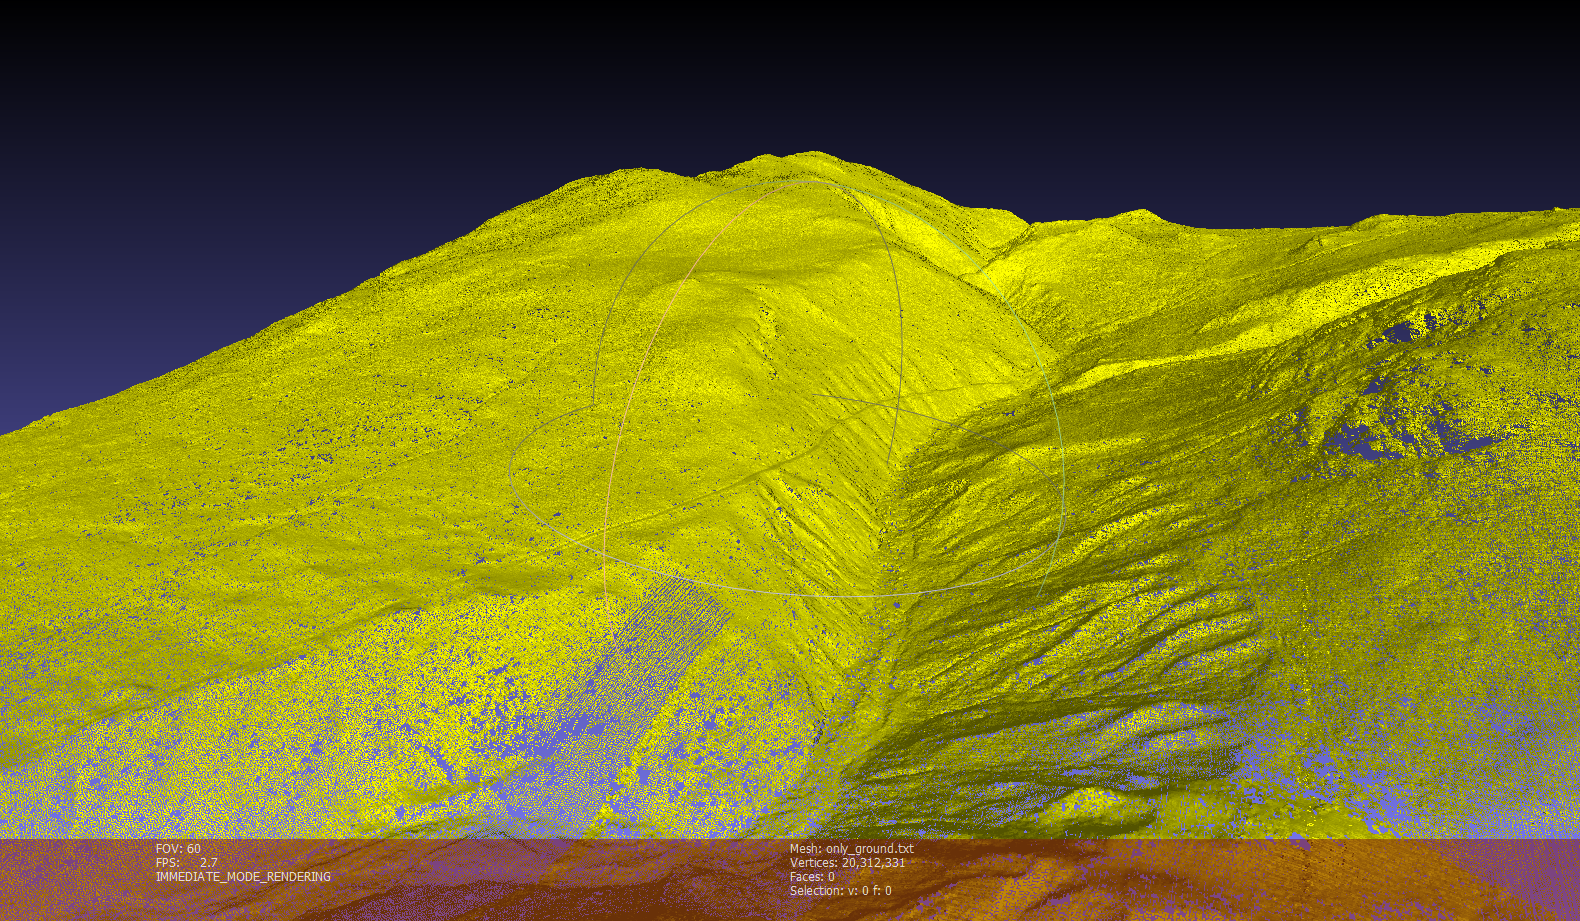
\includegraphics[width=\ImageWidth]{figures/point_cloud.PNG}
            \caption{Filtered Point Cloud for the Ground in the Vekveselva River Area}
            \label{fig:point_cloud}
        \end{figure}
        \FloatBarrier
        
        Screened Poisson Surface Reconstruction\cite{kazhdan2013screened} was used to recreate the ground model from the point cloud. It relies on the points having normals, so these normals had to be calculated first. The reconstructing algorithm was tested with different reconstructing depths where the choice landed on 12. This resulted in longer computing time but a very good reconstruction quality. The model was also cleaned for duplicate edges and vertices without normals.
        
        Because the ground model is constructed from points, and the points have gps coordinates, the resulting model has a very large offset from its local origin. Although a better practise would be to keep these coordinates, as they could be useful information later, they made it hard to locate the model in programs like Blender. Therefore the origin of the model was reset to approximately the centre of the geometry. The model was exported as a \texttt{.ply} file as it can be read by both Blender and Meshlab and has good compression.
    
    \subsection{Cut Model in Blender}
        Blender\cite{blender} is a versatile, open source software with many different features. It was used to further rework and texture the model where Meshlab proved less appropriate. It was first used to partition the model into three smaller areas that would be simplified at different rates. This partitioning can be seen in \cref{fig:model_original}. The reasoning behind the partition is to cut the model into the part that the player will move on, the are they will look at most, and the part they are only supposed to view at a distance or not at all. This will also allow parts of the model to be worked on in isolation from the rest.
        
        \FloatBarrier
        \begin{figure}[htbp]
            \centering
            \includegraphics[width=\ImageWidth]{figures/model_original.PNG}
            \caption{Partitioning of the Model Before Simplification}
            \label{fig:model_original}
        \end{figure}
        \FloatBarrier
        
        \todo{Update partition image}
    
    \subsection{Simplify Model in Meshlab}
        With the model divided into different parts, they can be simplified tailored to their importance. The Quadratic Edge Collapse Decimation algorithm was used to achieve this. This simplification allows to preserve the general topology, as well as the edges of the final model. This is important as the different parts of the model need to fit together at the end. The simplification was controlled by stating the percentage of vertices that should survive. Different percentages was tested for the ground models, to trade off quality against file size. As the models had a very high vertex count, the walkway was scaled to 15 \% of original vertex count, the main area was set to 2 \% and the rest were set to 0.1 \%.
        
        \todo{Input image of post-simplification}
    
    \subsection{Rework and Texture Model in Blender}
        Although the recreation of the walkway was successful, the omnidirectional treadmill needs more space than a person would normally need. This is because it is less precise than actual walking, as well as a little harder to control. To accommodate this the walkway was reworked in Blender to provide a flatter surface for the players. When the three ground models were ready, they were textured using a satellite image from Google Maps. Finally the ground models were exported as \texttt{.fbx} files, as Unity does not support the \texttt{.ply} format.
        
        \todo{Input image of post rework}

\section{Implementation in Unity}
    % How stuff was made in Unity, potentially code snippets.
    \subsection{Viewing Stereoscopic 360 Images}
    
    \subsection{Decorating the Game World}

\section{Achieved Milestones}
    % A table documenting achieved milestones: when and what
    To document the progress, different milestones with dates are noted in the following table:
    
    \FloatBarrier
    \begin{table}[htbp]
        \centering
        \begin{tabular}{|c|p{0.8\linewidth}|}
            \hline
            \textbf{Date} & \textbf{Milestone} \\
            \hline
            2020-01-15 & Meeting with domain experts to show progress and plans \\
            2020-02-04 & Finished ground models \\
            2020-02-06 & Meeting with domain expert to discuss interaction elements and content to be included \\
            2020-02-13 & Supervisor meeting to discuss research questions and gameplay elements \\
            2020-02-25 & \todo{User testing with geography students} \\
            2020-02-\todo{?} & \todo{Domain expert test of images} \\
            \hline
        \end{tabular}
        \caption{Achieved milestones}
        \label{tab:milestones}
    \end{table}
    \FloatBarrier

\chapter{Results}
\label{chap:results}

\section{Questionnaires}
    % Graphs of what people answered on the questionnaires, as well as explaining how the they were conducted.

\section{Interviews}
    % What was said by the different participators.
    
\chapter{Discussion}
\label{chap:discussion}

\section{Recreating Landscape from LiDAR}

\section{The Process for Creating a Virtual Field Trip}

\section{Advanced vs Simple Virtual Field Trip}

\todo{Evaluation/discussion of project, process and application here or in conclusion or both?}

\chapter{Conclusions and Future Work}
\label{chap:conclusion}

\section{Conclusion}

This is where you provide an overview of the thesis now that it is finished.  What are the critical things that can be learnt from the thesis for the reader.

This is additional text.

\section{Future Work}
\label{sec:future}
Where would the project go from here.

Investigate more automatic surface reconstruction

Create better game with more interactivity

Create app/level for preparation and afterwork

Perform actual user testing

Better tutorial for pointing and selecting


\printbibliography

%% First paper

% \begin{paper}{papers/landes1951scrutiny.pdf}{paper:scrutiny}
%     Here, you may add a description of the paper, an illustration, or just give the bibliographic reference:
%     \begin{quote}
%         \fullcite{landes1951scrutiny}
%     \end{quote}
%     Or you may leave it empty, if you like.
% \end{paper}

% Second paper etc.

\appendix
%% \chapter{Additional Material}
% \label{app:additional}

% Additional material that does not fit in the main thesis but may still be relevant to share, e.g., raw data from experiments and surveys, code listings, additional plots, pre-project reports, project agreements, contracts, logs etc., can be put in appendices. Simply issue the command \texttt{\textbackslash appendix} in the main \texttt{.tex} file, and make one chapter per appendix.

% If the appendix is in the form of a ready-made PDF file, it should be supported by a small descriptive text, and included using the \texttt{pdfpages} package. To illustrate how it works, a standard project agreement (for the IE faculty at NTNU in Gjøvik) is attached here. You would probably want the included PDF file to begin on an odd (right hand) page, which is achieved by using the \texttt{\textbackslash cleardoublepage} command immediately before the \texttt{\textbackslash includepdf[]\{\}} command. Use the option \texttt{[pages=-]} to include all pages of the PDF document, or, e.g., \texttt{[pages=2-4]} to include only the given page range.

% \cleardoublepage
% \includepdf[pages=-]{appendices/NTNUProsjektavtale.pdf}

\end{document}